\begin{figure}
    \begin{center}
    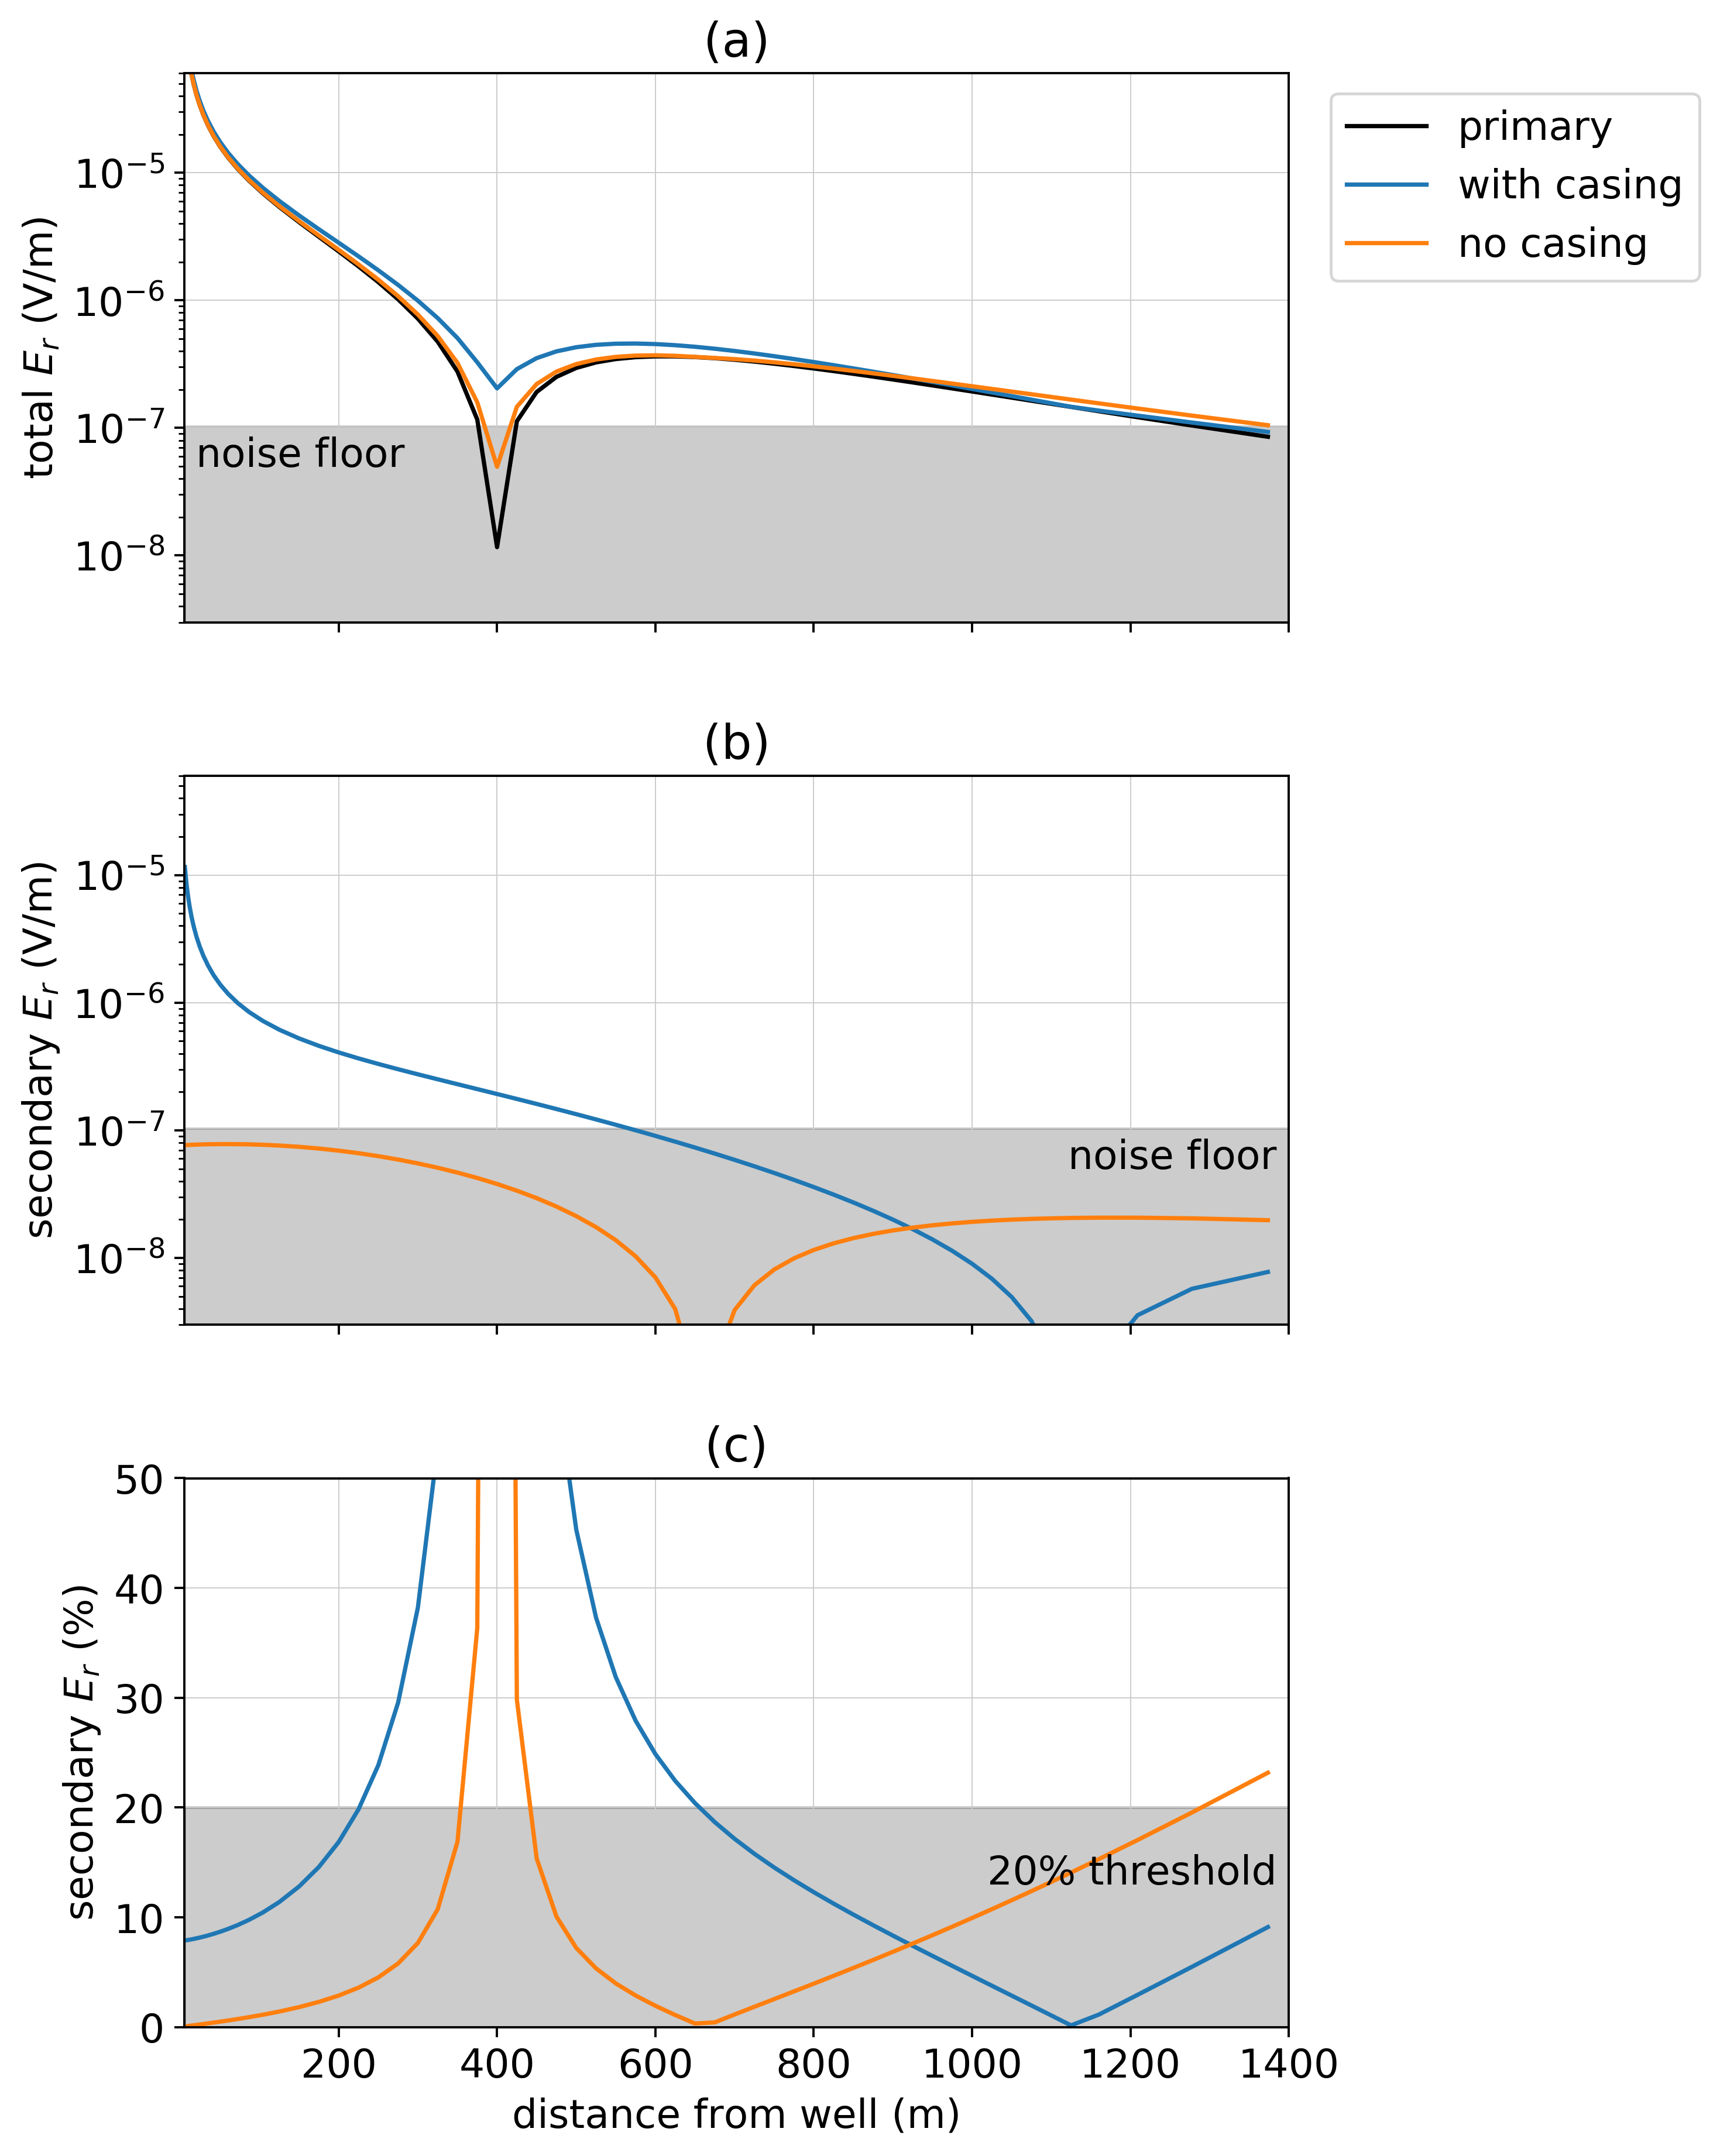
\includegraphics[width=0.8\textwidth]{figures/dc_casing/detectability_dipole.png}
    \end{center}
\caption{
    (a) Sum of the primary and secondary radial electric field due to a dipolar
    target with moment of 38 Am
    centered 50 m from the well, either calculated with the
    casing (blue) or simply a dipole in a half-space (orange). (b) Secondary
    radial electric field due to a dipolar target in a halfspace with casing (blue) and without casing (orange).
    Secondary radial electric field as a percentage of the primary.
    The target is along a line $90^\circ$ from the
    source electrodes; this is the same line along which we measure data at the surface.
}
\label{fig:detectability_dipole}
\end{figure}
